% created for PPSN conference http://ppsn2006.raunvis.hi.is/
% Time-stamp: "2006-09-12 05:40:55 tpr"
% PAPER PPSN-
% if all fonts computer modern use -G1
% dvips -Ppdf -G0 <filename>
% http://www.springer.de/comp/lncs/authors.html
% http://geneura.ugr.es/~jmerelo/ppsn2004/author.cgi?Information=1&authorID=947&password=seathe
% name: Thomas Philip Runarsson
% e-mail: tpr@hi.is

\documentclass[10pt]{llncs}
\usepackage[english]{babel}
\usepackage{latexsym}
\usepackage{times}
\usepackage{amsmath,amssymb}
\usepackage[dvips]{graphicx,psfrag}

\newcommand{\norm}[1]{\lVert#1\rVert}
\renewcommand{\vec}[1]{{\mbox{\boldmath$#1$}}}
\newcommand{\mat}[1]{{\mbox{\boldmath$#1$}}}
\newcommand{\reals}{{\mathbb R}}
\newcommand{\strng}[1]{{\mbox{\tt #1}}}
\newcommand{\inner}[2]{\big<\vec{#1}\cdot\vec{#2}\big>}

\def\argmax{\mathop{\rm argmax}}
\def\argmin{\mathop{\rm argmin}}
\newcommand\bs{\char '134}   

%\newcommand{\mat}[1]{{\mathbf #1}}
\renewcommand{\vec}[1]{{\mathbf #1}}
%\setlength{\textheight}{9.1in} \setlength{\topmargin}{0in} % was 9.3in
%\setlength{\oddsidemargin}{0.18in}\setlength{\evensidemargin}{0.18in}
%\addtolength{\textwidth}{0.2\textwidth}
\hyphenpenalty=800
\hbadness=2500

\title{Ordinal Regression in Evolutionary Computation}

\author{Thomas Philip Runarsson}
\institute{{Science Institute, University of Iceland}\\
\email{tpr@hi.is}}
\begin{document}
\maketitle

%\thispagestyle{empty}\pagestyle{empty}
\selectlanguage{english}

\begin{abstract}
  Surrogate ranking in evolutionary computation using ordinal
  regression is introduced. The fitness of individual points is
  indirectly estimated by modeling their rank. The aim is to
  reduce the number of costly fitness evaluations needed for
  evolution. The ordinal regression, or preference learning,
  implements a kernel-defined feature space and an optimization
  technique by which the margin between rank boundaries is
  maximized.  The technique is illustrated on some classical
  numerical optimization functions using an evolution strategy.
  The benefits of surrogate ranking, compared to surrogates that
  model the fitness function directly, are discussed.
\end{abstract}

\section{Introduction}\label{sec:introduction}

Evolutionary computation is a biologically inspired iterative
process where a population of search points is produced
generation after generation. Through parent points a typical
evolutionary algorithm will generate a number of new candidate
points by reproduction, recombination and mutation. The best of
these points will replace some if not all parent points through
a selection process. The selection process generally uses an
objective function similar to that used in classical methods of
search and optimization. In this case the function is referred
to as the fitness function. However, unlike classical
optimization techniques, the method for selecting the best
candidates in evolutionary computation requires only the rank
(or partial rank) of the candidates\footnote{The exception is
  fitness proportionate selection which is rarely used in
  practice.}.  Alternatively the selection process may be the
result of co-evolution where individual points compete for
reproduction.  In this case there is no explicit fitness
function defined, but rather an indirect method of evaluating
whether one point is preferable to another.

The current approach in fitness approximation for evolutionary
computation involves building surrogate fitness models directly
using regression.  For a recent review of the state-of-the-art
see \cite{Ong04,SLK05,Jin05}.  The fitness model is based on a
set of evaluated points called the training set. The surrogate
model is used to predict the fitness of candidate search points.
Commonly a fraction of points are selected and evaluated within
each generation (or over some number of generations
\cite{JOS02}), added to the training set, and used for updating
the surrogate.  The goal is to reduce the number of costly true
fitness evaluations while retaining a sufficiently accurate
surrogate during evolution. Direct models of the fitness
function are only possible when a fitness function can be
defined.  Current methods are therefore unsuitable for
co-evolution and interactive evolution.  For example,
co-evolution has been used to evolve game playing strategies,
where two or more strategies compete by playing a number of
games against each other.  In interactive evolution a human
user may be used to rank candidate points.  The approach
presented here, based on ordinal regression, is applicable to
the cases where no explicit or computable fitness function is
available.

In evolutionary computation the surrogate approach should be
considered as a preference learning task, where a candidate
point $\vec{x}_i$ is said to be preferred over $\vec{x}_j$ if
$\vec{x}_i$ has a higher fitness than $\vec{x}_j$. The training
set for the surrogate model is therefore composed of pairs of
points $(\vec{x}_i,\vec{x}_j)_k$ and a corresponding label
$t_k\in[1 ,-1]$, taking the value $+1$ (or $-1$) when
$\vec{x}_i$ has a higher fitness than $\vec{x}_j$ (or vice
versa).  The direct fitness approximation approach does not make
full use of the flexibility inherent in the ordering
requirement.  In classical optimization regression is necessary
when the method of search is gradient based, see for example
\cite{Madsen04}.  Evolutionary optimization is a stochastic and
direct search method where only the full or partial ordering of
the search points is needed.  For this reason an ordinal
regression offers sufficiently detailed surrogates for
evolutionary computation.

The technique presented for ordinal regression is kernel based.
This implies that the technique can be readily applied to
different data types as long as a kernel can be defined.  For
example, the search points may be represented by a tree or
variable length strings. Section~\ref{sec:OR} describes the
method of ordinal regression using kernel-defined features.  The
technique is illustrated and tested in section~\ref{sec:MS}
using various kernels to fit Rosenbrock's function. In
section~\ref{sec:MI} a strategy for updating the surrogate
during search is discussed and its effectiveness illustrated
using the CMA-ES \cite{hansen:ostermeier:01} on some numerical
optimization functions.  This is followed by a discussion 
and conclusion.


\section{Ordinal Regression}\label{sec:OR}

The preference learning task of ordinal regression presented
here is a variation of the work presented in
\cite{Herbrich00,joachims02}. The modification relates to how
the point pairs are selected and the fact that a $2-$norm soft
margin support vector machine (SVM) is used\footnote{Initial
  experiments using the $1-$norm soft margin SVM were not
  entirely satisfactory. This was found to be due to the
  quadratic programming solver used in the experiments (the
  PR\_LOQO optimizer by A. Smola).}. The training pairs are
selected to reflect the fact that a full ranking surrogate model
is required for the work presented here. It is also possible to
select the pair by random sampling as is done in \cite{Herbrich00}.

The ranking problem is specified by a set $S =
\{(\vec{x}_i,y_i)\}_{i=1}^\ell \subset X \times Y$ of point/rank
pairs, where $Y=\{r_1,\ldots,r_\ell\}$ is the outcome space with
ordered ranks $r_1> r_2,> \ldots > r_\ell$.   Now consider the model space
$\mathcal{H} = \{h(\cdot) : X \mapsto Y\}$ of mappings from points to
ranks. Each such function $h$ induces an ordering $\succ$ on the
points by the following rule:
\begin{equation}
\vec{x}_i \succ \vec{x}_j \quad \Leftrightarrow \quad
h(\vec{x}_i) > h(\vec{x}_j)
\end{equation}
where the symbol $\succ$ denotes ``is preferred to''.  In
ordinal regression the task is to obtain function $h^*$ that can
for a given pair $(\vec{x}_i,y_i)$ and $(\vec{x}_j,y_j)$
distinguish between two different outcomes: $y_i > y_j$ and $y_j
> y_i$. The task is therefore transformed into the problem of
predicting the relative ordering of all possible pairs of
examples \cite{Herbrich00,joachims02}.  However, it is
sufficient to consider only all possible pairs of adjacent
ranks, see also \cite{shawe-taylor04:book} for yet an
alternative formulation.  The training set, composed of pairs,
is then as follows:
$$S' = \big\{(\vec{x}_k^{(1)},
\vec{x}_k^{(2)}),t_k=\text{sign}(y_k^{(1)} -
y_k^{(2)})\big\}_{k=1}^{\ell'}$$
where $(y_k^{(1)} = r_i) \wedge
(y_k^{(2)} = r_{i+1})$ (and vice versa $(y_k^{(1)} = r_{i+1})
\wedge (y_k^{(2)} = r_{i})$) resulting in $\ell'=2(\ell-1)$
possible adjacently ranked training pairs. The rank difference
is denoted by $t_k\in[-1,1]$.

In order to generalize the technique to different point data
types and model spaces an implicit kernel-defined feature space
with corresponding feature mapping $\phi$ is applied. Consider
the feature vector
$\phi(\vec{x})=[\phi_1(\vec{x}),\ldots,\phi_m(\vec{x})]^T\in
\reals^m$ where $m$ is the number of features. Then the
surrogate considered may be defined by a linear function in the
kernel-defined feature space:
\begin{equation}
h(\vec{x}) = \sum_{i=1}^m w_i\phi_i(\vec{x}) =
\inner{w}{\phi(\vec{x})}.
\end{equation}

The aim is now to find a function $h$ that encounters as few
training errors as possible on $S'$. Applying the method of
large margin rank boundaries of ordinal regression described in
\cite{Herbrich00}, the optimal $\vec{w}^*$ is determined by
solving the following task:
\begin{equation}
\min_{\vec{w}}\quad \tfrac{1}{2}\inner{w}{w} + \tfrac{C}{2}\sum_{k=1}^{\ell'}\xi_k^2
\label{eq:margin}
\end{equation}
subject to
$t_k\inner{w}{(\phi(\vec{x}_k^{(1)})-\phi(\vec{x}_k^{(2)})}\ge 1
- \xi_k$ and $\xi_k \ge 0$, $k = 1,\ldots, \ell'$. The degree
of constraint violation is given by the margin slack variable
$\xi_k$ and when greater than $1$ the corresponding pair are
incorrectly ranked. Note that
\begin{equation}
h(\vec{x}_i)-h(\vec{x}_j) = \inner{w}{(\phi(\vec{x}_i)-\phi(\vec{x}_j))}
\end{equation}
and that minimizing $\inner{w}{w}$ maximizes the margin between
rank boundaries, in our case the distance between adjacently
ranked pair $h(\vec{x}^{(1)})$ and $h(\vec{x}^{(2)})$.

In terms of the training data, the optimal $\vec{w}^*$ can be
expressed as:
\begin{equation}
\vec{w}^* = \sum_{k=1}^{\ell'}\alpha^*t_k\big(\phi(\vec{x}_k^{(1)})-\phi(\vec{x}_k^{(2)})\big)
\end{equation}
and the function $h$ may be reconstructed as follows:
\begin{eqnarray}
h(\vec{x}) = \big<\vec{w}^*\cdot\phi(\vec{x})\big> & = &
\sum_{k=1}^{\ell'}\alpha^*t_k\big(\big<\phi(\vec{x}_k^{(1)})\cdot\phi(\vec{x})\big>-\big<\phi(\vec{x}_k^{(2)})\cdot\phi(\vec{x})\big>\big)\nonumber\\
& = & \sum_{k=1}^{\ell'}\alpha^*t_k\big(\kappa(\vec{x}_k^{(1)},\vec{x})-\kappa(\vec{x}_k^{(2)},\vec{x})\big)
\end{eqnarray}
where $\kappa(\vec{x},\vec{z}) =
\inner{\phi(\vec{x})}{\phi(\vec{z})}$ is the chosen kernel and
$\vec{\alpha}^*_k$ are the Lagrangian multipliers for the
constraints that can be determined by solving the dual quadratic
programming problem:
{
\begin{eqnarray}
%\ & \max_{\vec{\alpha}}\quad \sum_{k=1}^{\ell'}\alpha_k-\tfrac{1}{2}\sum_{i=1}^{\ell'}\sum_{j=1}^{\ell'}\alpha_i\alpha_jt_it_j\big((\phi(\vec{x}_i)^{(1)}-\phi(\vec{x}_i^{(2)}))\cdot(\phi(\vec{x}_j)^{(1)}-\phi(\vec{x}_j^{(2)}))+\tfrac{1}{C}\delta_{ij}\big)\nonumber\\
 \max_{\vec{\alpha}} \quad
\sum_{k=1}^{\ell'}\alpha_k-\tfrac{1}{2}\sum_{i=1}^{\ell'}\sum_{j=1}^{\ell'}\alpha_i\alpha_jt_it_j\big( K(\vec{x}_i^{(1)},\vec{x}_i^{(2)},\vec{x}_j^{(1)},\vec{x}_j^{(2)})+\tfrac{1}{C}\delta_{ij}\big)
\end{eqnarray}}
subject to $\sum_{k=1}^{\ell'}\alpha_kt_k=0$ and $0\le \alpha_k$, $k =
1,\ldots,\ell'$, where
$K(\vec{x}_i^{(1)},\vec{x}_i^{(2)},\vec{x}_j^{(1)},\vec{x}_j^{(2)}) =
\kappa(\vec{x}_i^{(1)},\vec{x}_j^{(1)})-\kappa(\vec{x}_i^{(1)},\vec{x}_j^{(2)})-\kappa(\vec{x}_i^{(2)},\vec{x}_j^{(1)})+\kappa(\vec{x}_i^{(2)},\vec{x}_j^{(2)})$,
where $\delta_{ij}$ is the Kronecker $\delta$ defined to be $1$ if
$i=j$ and $0$ otherwise \cite{CS02:book}. 

The following section illustrates the technique on a simple
problem using common kernels. It is also discussed how the
accuracy of the surrogate is evaluated.

\section{Model Selection}\label{sec:MS}

Model selection in surrogate ranking involves choosing a kernel
and it parameters. Furthermore, the regulation parameter $C$ in
\eqref{eq:margin} controlling the balance between model
complexity and training errors must be chosen appropriately.  A
suitable kernel choice is problem specific. For example,
consider Rosenbrock's function
\begin{equation}
f(\vec{x}) = \sum_{i=2}^n 100(x_{i}-x_{i-1}^2)^2 + (1-x_{i-1})^2
\end{equation}
whose optimal point is located at $\vec{x} = (1,\ldots,1)$.
Rosenbrock's function is a fourth order polynomial and so the
\emph{polynomial kernel}
\begin{equation}
\kappa(\vec{x}_i,\vec{x}_j) = (1 + \inner{x_i}{x_j})^d
\end{equation}
of order $d=4$ may seem appropriate. Quadratic approximations are
also commonly used in local optimization and so a polynomial kernel
with $d=2$ could also be an interesting alternative. However, perhaps the most 
commonly used kernel in the literature is the \emph{Gaussian kernel},
\begin{equation}
\kappa(\vec{x}_i,\vec{x}_j) = \exp\big(-\gamma \norm{\vec{x}_i-\vec{x}_j}^2\big).
\end{equation}
When applying kernel methods it is also important to scale the
points $\vec{x}$ first. A standard method of doing so is to
scale the training set such that all points are in some range,
typically $[-1,1]$. That is, scaled $\tilde{\vec{x}}$ is
\begin{equation}
\tilde x_i = 2 (x_i - \underline{x}_i) / (\overline{x}_i -
\underline{x}_i) - 1 ~~~ i = 1,\ldots,n
\end{equation}
where $\underline{x}_i$, $\overline{x}_i$ are the maximum and
minimum values of variable $i$ in set $S$. Scaling makes it
easier to fix $C$ and kernel parameters during evolution. This
is especially important as the evolutionary search zooms in on a
particular region of the search space.

Let $n=2$ and $S=\big\{\vec{x}_i,y_i\big\}_{i=1}^\ell$ be the
$\ell$ training points sampled using a standard normal
distribution centered about the origin for Rosenbrock's
function.  Using $\ell = 10, 20, \ldots, 60$ randomly sampled
training points the surrogate model $h$ is estimated by ordinal
regression. The $h$ contour plots for the extreme cases
$\ell=10$ and $\ell=60$ and the three different kernels are
depicted in Fig.~\ref{fig:Rosenbrock}.  The contours of
$f(\vec{x})$ are given by the dotted lines in each case.  The
sampled training points are depicted by dots. In the case of a
4th order polynomial and RBF kernel the training accuracy is
100\% for the $2(\ell-1)$ adjacently ranked point pairs, when
$C=1E6$.  However, regardless of how high $C$ is set for the 2nd
order polynomial kernel a training accuracy of around 50\% is
consistently observed. This can be used as an indicator that the
current kernel-defined features are not powerful enough to
describe the ranking. On the other hand the RBF and 4th order
polynomial kernel may overfit the training data. An example of
this can be seen in Fig.~\ref{fig:Rosenbrock} (top) when $\ell=10$.
However, as the number of training samples increase the chance
of overfitting decreases as seen in Fig.~\ref{fig:Rosenbrock}
(bottom).

\begin{figure}[t!]
%\centering
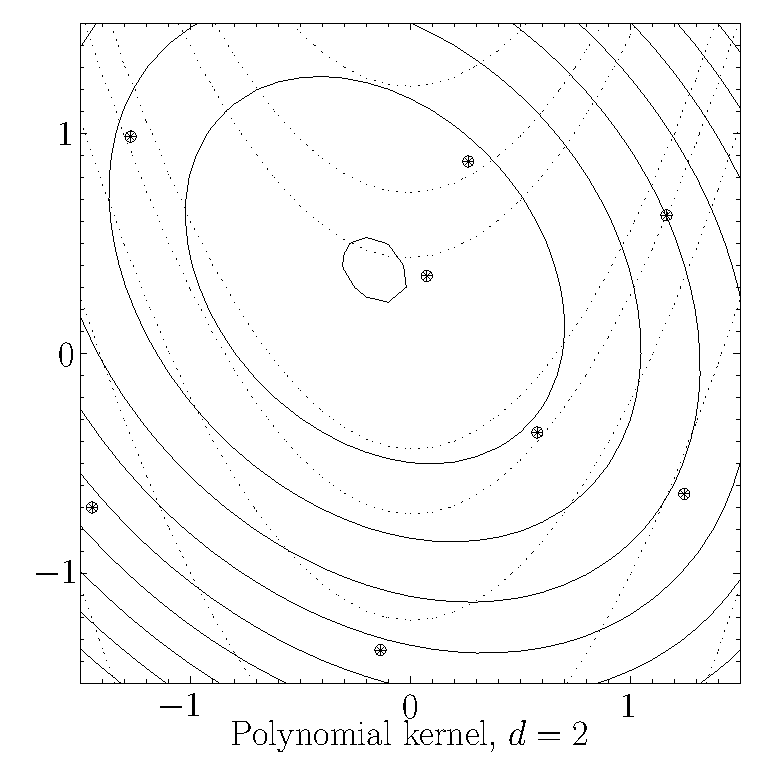
\includegraphics[height=0.33\columnwidth]{figs/poly2global10.eps}
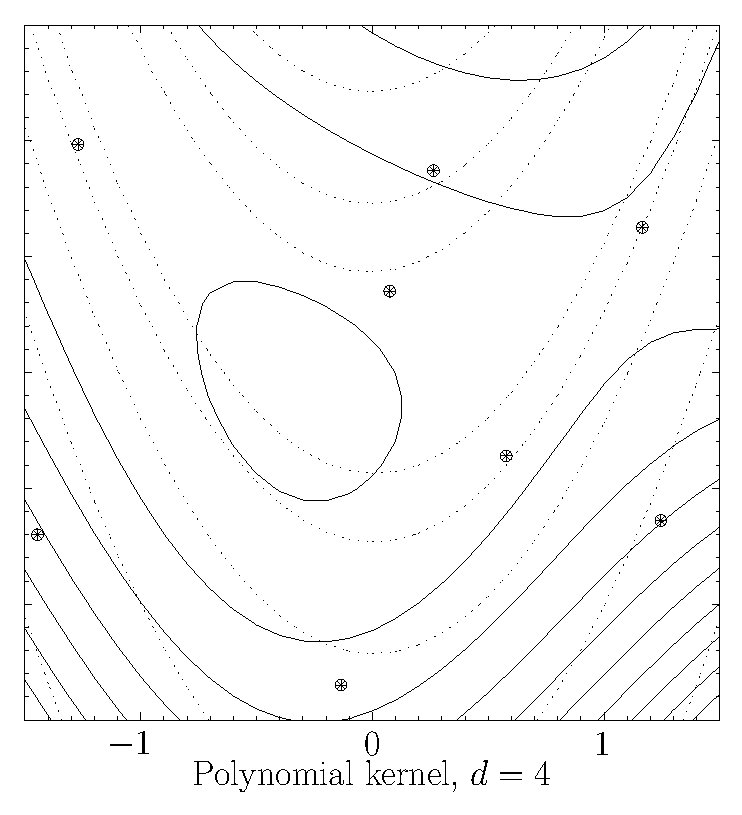
\includegraphics[height=0.33\columnwidth]{figs/poly4global10.eps}
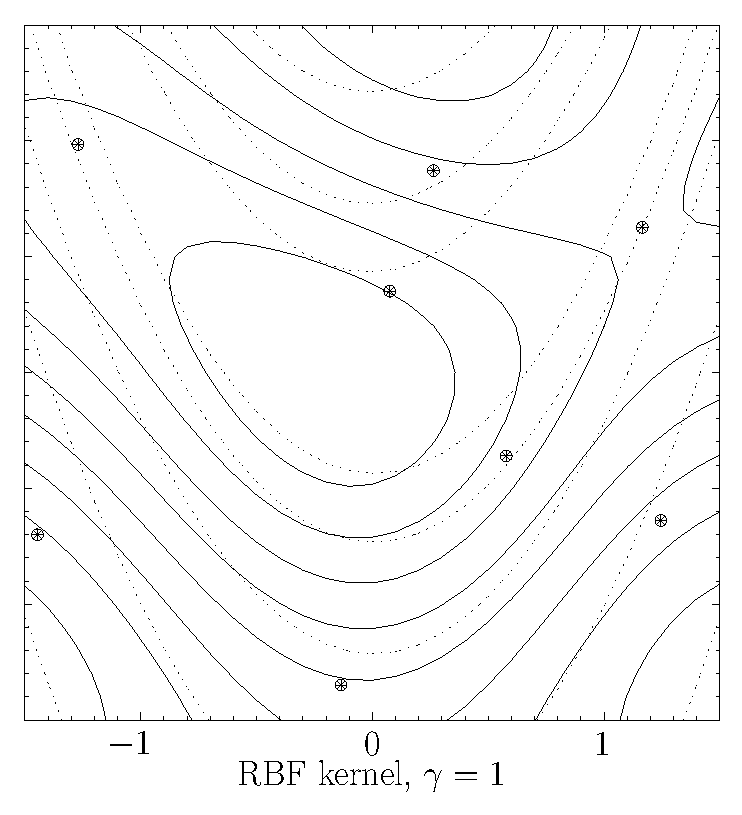
\includegraphics[height=0.33\columnwidth]{figs/rbf1global10.eps}\\
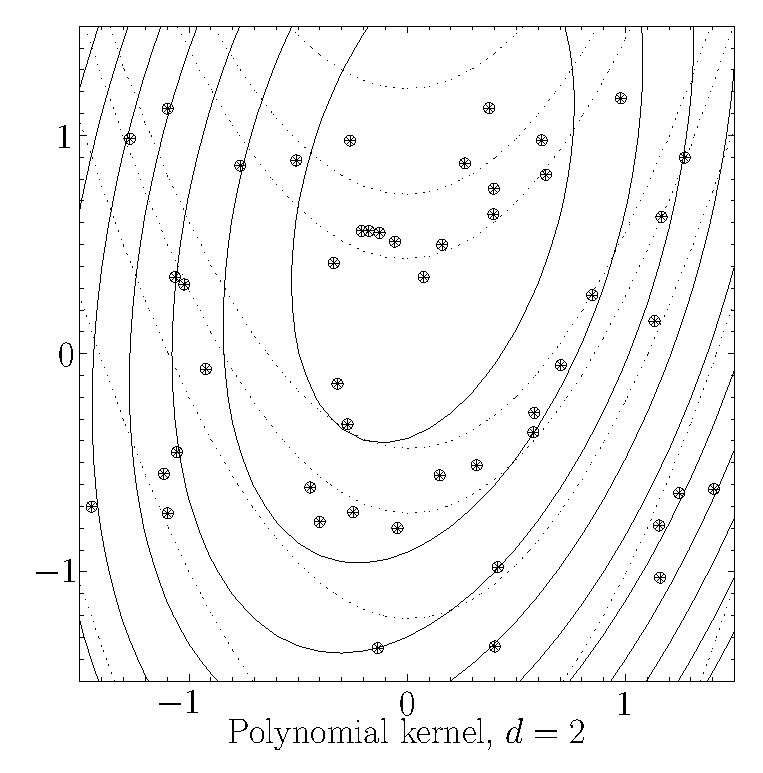
\includegraphics[height=0.33\columnwidth]{figs/poly2global.eps}
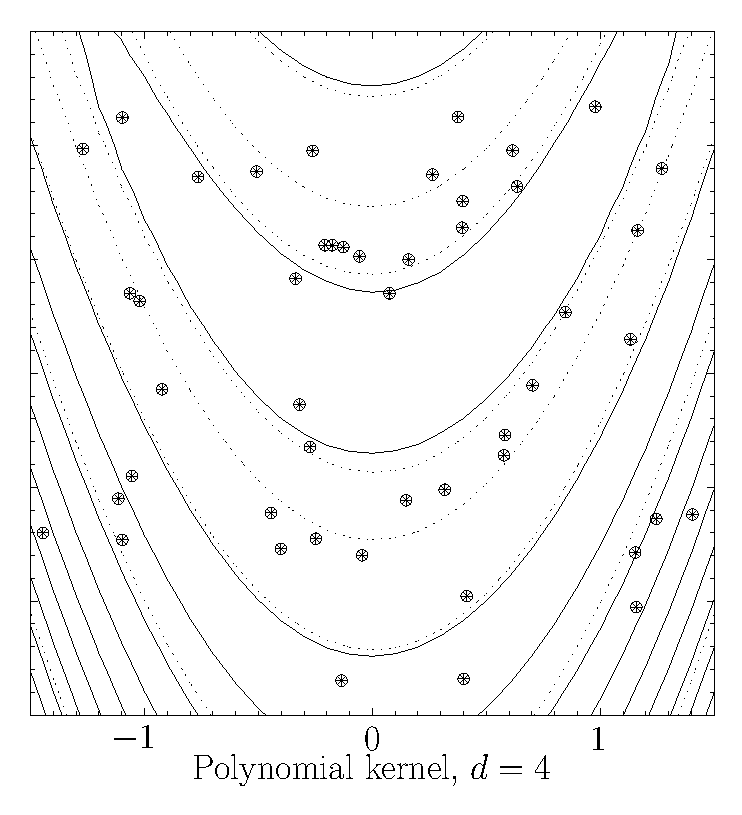
\includegraphics[height=0.33\columnwidth]{figs/poly4global.eps}
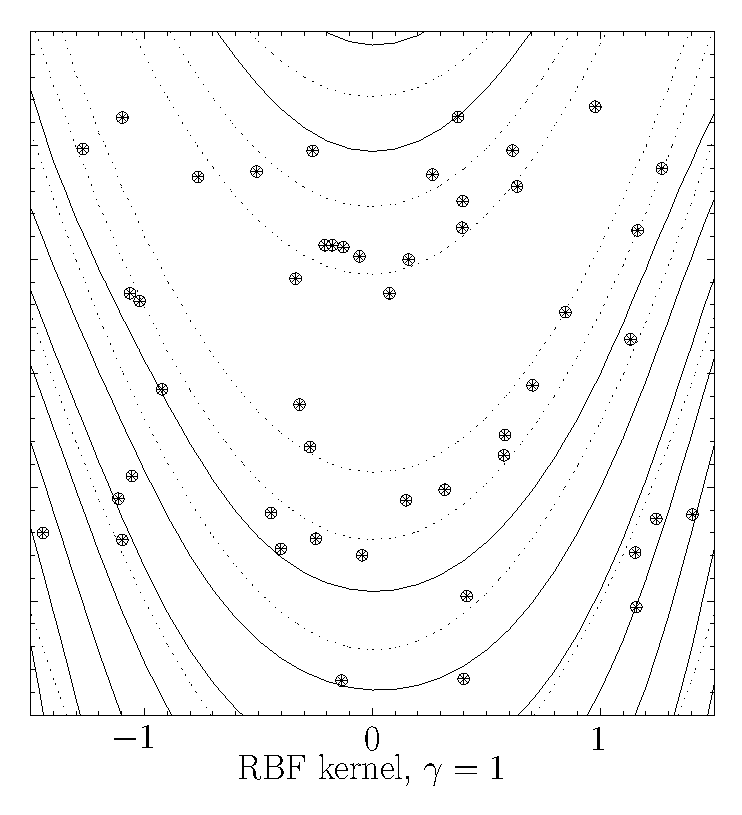
\includegraphics[height=0.33\columnwidth]{figs/rbf1global.eps}
\caption{Contour plots of the true function (dotted lines)
  versus surrogate (solid lines) for the three different
  kernels. The $\ell=10$ (top) and $\ell=60$ (bottom) training
  points are depicted as dots.}
\label{fig:Rosenbrock}
\end{figure}

%% \begin{figure}[t!]
%% %\centering
%% 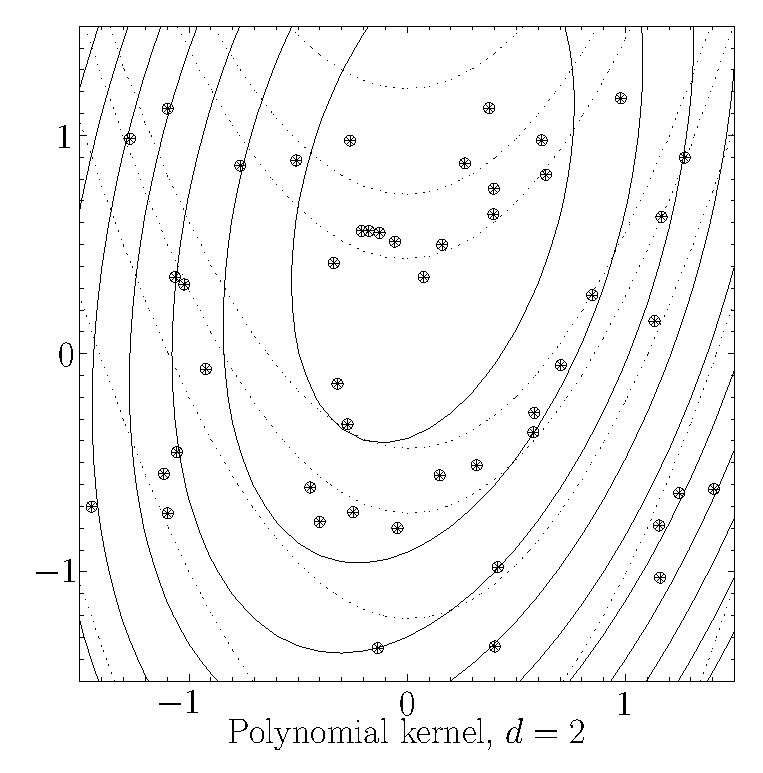
\includegraphics[height=0.33\columnwidth]{figs/poly2global.eps}
%% 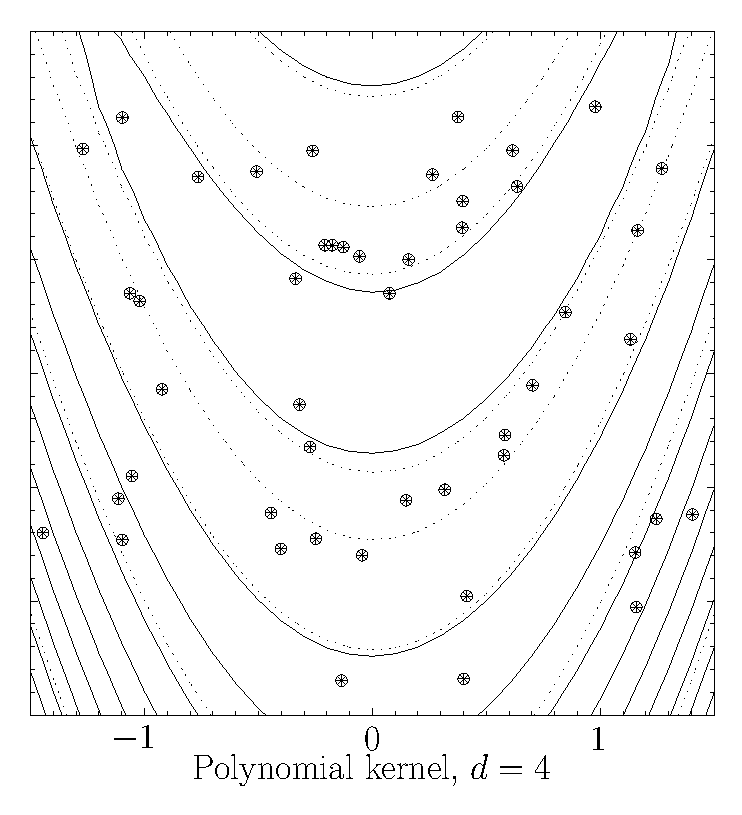
\includegraphics[height=0.33\columnwidth]{figs/poly4global.eps}
%% 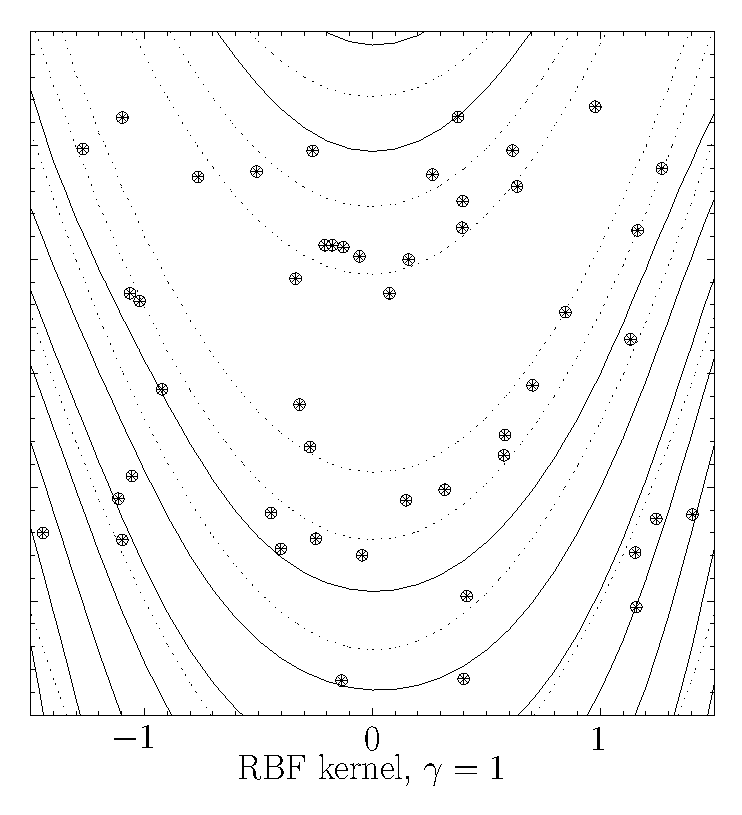
\includegraphics[height=0.33\columnwidth]{figs/rbf1global.eps}
%% \caption{Contour plots of the true function (dotted lines)
%%   versus surrogate (solid lines) for the three different
%%   kernels. The $\ell=60$ training points are depicted as dots.}
%% \label{fig:Rosenbrock60}
%% \end{figure}

When the training accuracy is 100\% one way of evaluating the
accuracy of the surrogate is through cross validation. The
quality of the surrogate is measured as the rank correlation
between the surrogate ranking and the true ranking on test data.
Here Kendall's $\tau$ is used for this purpose.  Kendall's
$\tau$ is computed using the relative ordering of the ranks of all
$\ell(\ell-1)/2$ possible pairs.  A pair is said to be
concordant if the relative ranks of $h(\vec{x}_i)$ and
$h(\vec{x}_j)$ is the same for $f(\vec{x}_i)$ and
$f(\vec{x}_j)$, otherwise they are discordant.
 Kendall's $\tau$ is
the normalized difference in the number of concordant and
discordant pairs.
%% Kendall's $\tau$
%% is then defined as follows,
%% {\footnotesize
%% \begin{equation*}
%% \tau = \frac{\text{\#concordant}-\text{\#discordant}}{\sqrt{\text{\#concordant}+\text{\#discordant}+\text{\#ties$(h)$}}\sqrt{\text{\#concordant}+\text{\#discordant}+\text{\#ties$(f)$}}}
%% \end{equation*}}
Two rankings are the same when $\tau=1$, completely reversed if
$\tau = -1$, and uncorrelated for $\tau \approx 0$.

For our experiment the testing data is created in the same
manner as the training data.  The testing points are $1000$ in
total and Kendall's $\tau$ computed based on surrogates built
using $\ell=10,20,\ldots,60$ training points. Kendall's $\tau$
for this study is presented in Table~\ref{tbl:Rosenbrock} (left)
for the all three kernels along with the training accuracy. As
anticipated the model accuracy increases with $\ell$ and the 4th
order polynomial kernel appears most suitable.

\begin{table}[t!]
\centering
\caption{Kendall's $\tau$ for surrogate ranking versus
  true ranking of $1000$ testing points generated around point
  $\vec{x}=[0,0]$ and  $\vec{x}=[1,1]$ in Rosenbrock's function for various kernels $\kappa$ and number of
  training points $\ell$.}
\label{tbl:Rosenbrock}
{\footnotesize
\begin{tabular}{|c|cccccc||cccccc|}
\hline
$\kappa$\quad\quad\quad\quad\quad$\ell=$ & $10$ & $20$ & $30$ & $40$ & $50$ & $60$ & $10$ & $20$ & $30$ & $40$ & $50$ & $60$  \\
\hline
& &  $\vec{x}$ & $=$  & $[0,0]$ & & & & $\vec{x}$ & $=$  & $[1,1]$ & &  \\

\hline
Polynomial, $d=2$ & $0.67$ & $0.66$ & $0.67$ & $0.65$ & $0.63$ & $0.60$ & $0.77$ & $0.94$ & $0.93$ & $0.91$ & $0.93$ & $0.93$\\
Training accuracy \% & $56$ & $58$ & $59$ & $59$ & $47$ & $49$ & $100$ & $100$ & $90$ & $69$ & $69$ & $71$ \\
\hline
Polynomial, $d=4$ & $0.59$& $0.88$ & $0.90$ & $0.98$ & $0.97$ & $0.98$ & $0.64$ & $0.83$ & $0.90$ & $0.93$ & $0.97$ & $0.98$\\
Training accuracy \% & $100$ & $100$ & $100$ & $100$ & $100$ & $100$ & $100$ & $100$ & $100$ & $100$ & $100$ & $100$ \\
\hline 
RBF, $\gamma=1$ & $0.65$ & $0.85$ & $0.90$ & $0.91$ & $0.93$ & $0.96$ & $0.73$ & $0.84$ & $0.91$ & $0.92$ & $0.94$ & $0.97$ \\
Training accuracy \% & $100$ & $100$ & $100$ & $100$ & $100$ & $100$ & $100$ & $100$ & $100$ & $100$ & $100$ & $100$ \\ 
\hline 
\hline
\end{tabular}}
\end{table}

As the search zooms in on a local minima one may expect that
different kernels may be suitable. The experiment is therefore
re-run, this time the training and testing samples are sampled
centered at the global minima from a Gaussian distribution with
variance $0.1^2$. In this case the 2nd order polynomial kernel
performs much better, even though the training accuracy is not
100\% for higher values of $\ell$, as shown in
Table~\ref{tbl:Rosenbrock} (right). Using Kendall's $\tau$ to
evaluate the surrogate ranking of test points forms the basis of
our model improvement method presented in the following section.


%\newpage
\section{Model Improvement}\label{sec:MI}

During evolution different regions of the space are sampled and
as a consequence the surrogate ranking model may be
insufficiently accurate for new regions of the search space. It
is therefore of paramount importance to validate the surrogate
during evolution. The accuracy can be validated by generating
test points in the new region similarly to the test points used
in the previous section. In particular one is interested in
validating the accuracy of the ranking of potential parent
points during evolution as they are critical for success
\cite{Ru04:PPSN}.

%\pagebreak
The proposed model validation and improvement strategy is as
follows:
\begin{enumerate}
\item Estimate the ranking of a population of points of unknown
  fitness using the current surrogate. Let the point with the
  highest ranking be a test point, $\vec{x}_t$. Rank this test
  point with respect to the points in the training set using the
  current surrogate.
\item Evaluate the test point using the true fitness function
  and evaluate its true rank among the training points. In the
  case where no explicit fitness function can be defined, the
  test point is evaluated by comparing it with selected points
  in the training set.
\item Compare the rankings by computing the rank
  correlation $\tau_k$ for the ranking in 1 and 2.
\item Add this new point to the training set.
\item If $\tau_k$ is equal to $1$ the model is said to be
  sufficiently accurate. This is a simple cross-validation on a
  single test point. Creating more test points would be too
  costly, but plausible.
\item If $\tau_k < 1$ the model is not sufficiently accurate. In
  this case update the surrogate using the new training set.
  Repeated the steps above until $\tau=1$ or all points of
  unknown fitness have been evaluated.
\end{enumerate}
The frequency by which the model is validated may be at each
generation or every $K>1$ generations. In this work the model is
validated at every generation. 

\begin{figure}[b!]
\centering
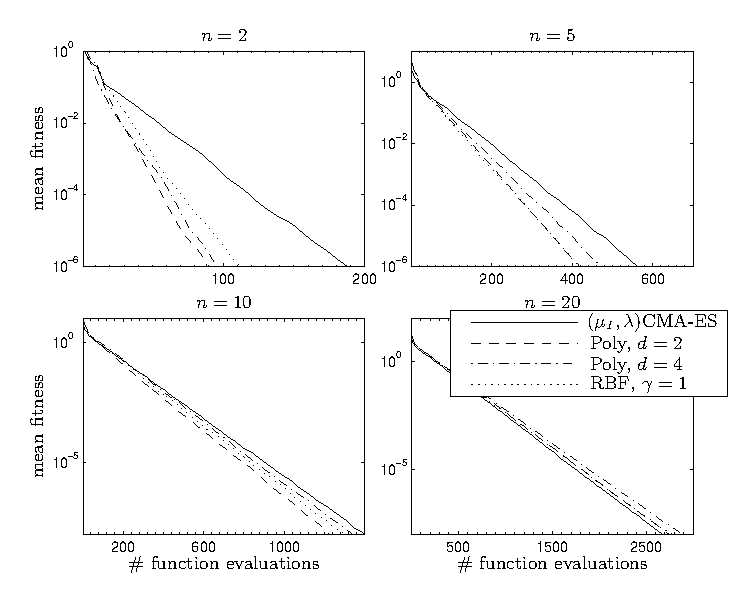
\includegraphics[width=0.8\columnwidth]{figs/sphere_1.eps}
\caption{Mean fitness values versus number of function
  evaluation for three different kernels and the original CMA-ES for
  different dimensions $n$ of the sphere model.}
\label{fig:sphere}
\end{figure}


Initially at least two known points, $\ell=2$, must be in the
training set for the ordinal regression to work. However, with
time the size of the training set grows without limit. In
evolutionary computing one is interested in the accurate ranking
of points generated in the neighborhood of parent points. If the
training set is to have a limited size $\overline{\ell}$ then it
would be reasonable to delete the oldest training points from
the set first. These deleted points are likely to be
representatives of a region of the search space which is no
longer of interest.


If the training accuracy is not 100\% then clearly $\tau_k < 1$.
In this case additional training points will be forced for
evaluation. It may be necessary to increase the value of $C$ in
order to improve training accuracy or alternatively to select
another kernel during search. Decreasing the size of the
training data set will also result in 100\% training accuracy
but at
the cost of overfitting.


\begin{figure}[t!]
\centering
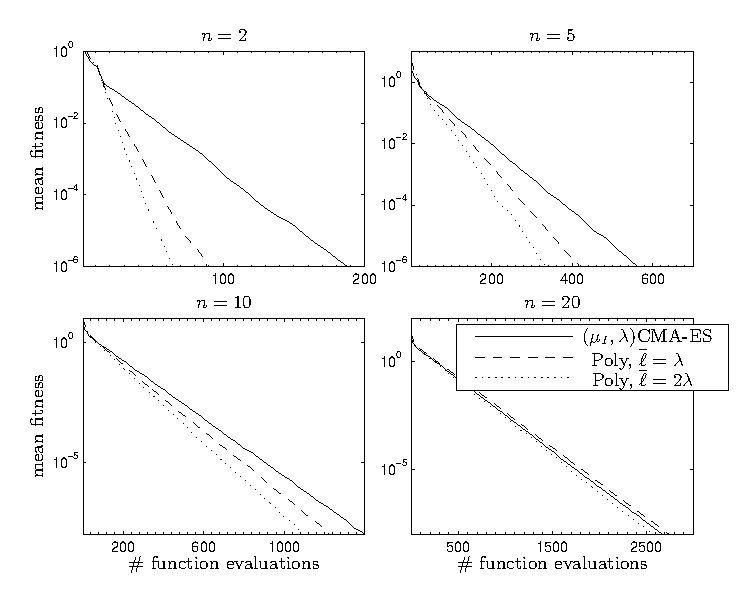
\includegraphics[width=0.8\columnwidth]{figs/sphere_2.eps}
\caption{The 2nd order polynomial kernel versus the original
  CMA-ES using $\overline{\ell}=\lambda$ and
  $\overline{\ell}=2\lambda$ for different dimensions $n$ of the sphere model.}
\label{fig:sphere2}
\end{figure}


The surrogate ranking validation and improvement strategy using
ordinal regression is now tested using the CMA-ES
\cite{hansen:ostermeier:01}. The CMA-ES is a very efficient
numerical optimization technique but we still expect to reduce
the number of function evaluations needed for search. The
average fitness for $100$ independent runs versus the number of
function evaluations are compared to the original CMA-ES for
various dimensions $n=2,5,10$ and $20$. The parameter setting
for the $(\mu_I,\lambda)$ CMA-ES is as recommended in
\cite{hansen:ostermeier:01} with population size $\lambda =
4+\lfloor 3\ln(n)\rfloor$ and the number of parents selected
$\mu=\lambda/4$. The stopping criteria used are $1000n$ function
evaluation or a fitness less than $10^{-10}$. The initial
mean search point is generated from a uniform distribution
between $0$ and $1$. Unless otherwise specified $\overline{\ell}
= \lambda$ and the training set is only pruned to size
$\overline{\ell}$ subsequent to the validation and improvement
procedure above. During model improvement the data scaling is
based on the current training set and new points to be ranked.
In all runs presented a 100\% training accuracy is achieved by
setting $C=1E6$.



The first experimental results are presented for the infamous
sphere model, $f(\vec{x}) = \sum_{i=1}^nx_i^2$. The average
fitness versus the number of function evaluations is presented
in Fig.~\ref{fig:sphere}. As one may expect for a quadratic
function, the 2nd order polynomial performs best. However, as
the dimensions increase the performance edge achieved by
surrogate ranking, over the original CMA-ES, is lost. The reason
for this is that a greater number of training samples are needed
at higher dimensions. To illustrate this trend the experiment is
repeated with $\overline{\ell} = 2\lambda$ using only the 2nd
order polynomial kernel. A comparison for the different problem
dimensions with the original CMA-ES and the case when
$\overline{\ell}=\lambda$ is shown in Fig.~\ref{fig:sphere2}.
The performance is improved in all cases when
$\overline{\ell}=2\lambda$ as expected.




The first experiment is now repeated but this time using
Rosenbrock's function for different dimensions. The traditional
CMA-ES will get stuck in local minima for this problem in around
4 out of 100 experiments. The polynomial kernels again have a
performance edge over the original CMA-ES, however, the RBF
kernel is more likely to get stuck in the local minima.
Overfitting is more of a problem in this case and the simple
model (2nd order polynomial kernel) is best at higher
dimensions. Clearly the choice of kernel and number of training
pairs will influence search performance.

\begin{figure}[t!]
\centering
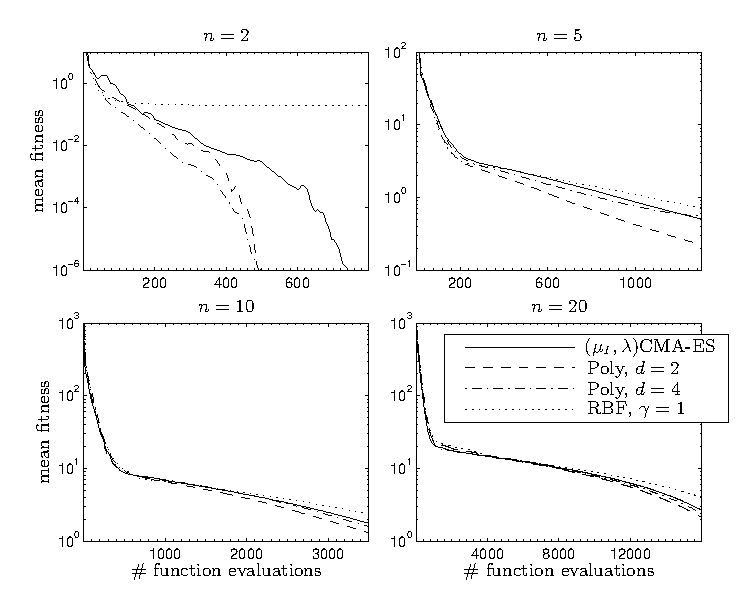
\includegraphics[width=0.8\columnwidth]{figs/rosen_1.eps}
\caption{Mean fitness values versus number of function
  evaluation for three different kernels and the original CMA-ES for
  different dimensions $n$ of Rosenbrock's function.}
\label{fig:rosen}
\end{figure}



%\pagebreak
\section{Discussion and Conclusion}\label{sec:Discussion}

When building surrogates in evolutionary computation one is
interested in the quality of ranking of points only. For this
reason the training accuracy and cross validation is a more
meaningful measure of quality for the surrogate model. This is in
contrast to regression, where the fitness function is modeled
directly and the quality estimated in terms of measures such a
the least square error. 

The technique used to control the number of true fitness
evaluations is based on a single test point. The ranking of this
test point using the current surrogate is compared with its true
ranking in order to determine the quality of the surrogate. This
is a simple form of cross-validation. An alternative approach
could be to rank all test points along with the training points
using the surrogate model. Then update the surrogate ranking
model using the single evaluated test point of highest rank.
This would then be followed by the re-ranking of training and
testing points using the updated surrogate and comparing it with
the previous estimate by computing Kendall's $\tau$. This style
of heuristic control was applied in \cite{Ru04:PPSN} with good
success. Its aim is to observe a change in ranking between
successive updates of the surrogate. In this case it may also be
sufficient for $\tau$ to be close to $1$ or at least the best
new candidate points (potential parent points) should be ranked
consistently.




%% To speed up ordinal regression one could use the previous
%% $\alpha$'s (corresponding to the old training points) and set
%% $\alpha = 0$ for new points, introduced to the training set, as
%% an initial setup for the quadratic programming problem.  An
%% additional strategy to pruning the training set is to keep only
%% those points which belong to a support vector pair
%% (characterized by $\alpha_k>0$).  Note that the number of
%% support vectors pairs also gives an upper limit on the leave one out
%% accuracy of the surrogate. This implies that when the number of
%% support vectors pairs is far less that $\ell'$ the surrogate
%% model should be more accurate.


%\section{Conclusion}

A generic framework for surrogate ranking using ordinal
regression in evolutionary computation has been presented. To
the best of our knowledge this is the first time such a
framework has been put forward. The formulation does not need an
explicitly defined fitness function, making it suitable for
co-evolution and interactive evolution. Choosing a
kernel-defined function $h$ also opens up the possibility of using
surrogates for other point data types. The only condition
is that a kernel can be defined.  For example, in genetic
programming a tree kernel may potentially be used. In
evolutionary art, kernels typically used in pattern recognition
may be useful.

The approach reduces the number of fitness evaluation needed,
without a loss in performance, as long as an appropriate kernel
is selected and a sufficient size of training data is available.
The studies presented are exploratory in nature and clearly the
approach must be evaluated on a greater range of evolutionary
tasks. These investigations are currently underway. 



%\newpage
\bibliographystyle{splncs}
\bibliography{biblio}

\end{document}

\begin{figure}[h!]
\centering \noindent 
{\footnotesize
\begin{tabbing}
\quad\quad\quad\quad\quad\quad\quad\quad\= 1 \ \emph{Initialize}: $\sigma = \sigma^* (r/n)$, $r = \norm{\vec{x}^*-\vec{x}_o}$\\
\> 2 \ {\bf for} $j := 1$ to $M$ {\bf do} \emph{(Monte Carlo Simulation)}\\ 
\> 3 \quad \= $\vec{z}_k = \vec{x}_o + \vec{N}_k(0,\sigma^2)$, $k=1\ldots,2$ \\
\> 4 \> evaluate the rank of $\vec{z}_k$, $k=1\ldots,2$\\
\> 5 \> $\vec{x}_i = \vec{x}_o + \vec{N}_i(0,\sigma^2)$, $i=1\ldots,\lambda$\\
\> 6 \> approximate $\hat{h}(\vec{x}_i)$ using \eqref{eq:nn} or \eqref{eq:knn}, $i=1\ldots,\lambda$\\
\> 7 \> $\varphi_j = r - \norm{\vec{x}^*-\vec{x}_{1:\lambda}}$\\
\> 8 \ {\bf od}\\
\> 9 \ Return \emph{expectation}: $\varphi^* = (n/r)\sum_{j=1}^M\varphi_j/M$\\
\end{tabbing}}
\caption{Model update procedure.}
\label{fig:Monte}
\end{figure}
